\section{Mendel,MD - Construção da Ferramenta}

A seguir apresentamos o software Mendel,MD, que foi desenvolvido para investigação dos casos clínicos recebidos pelo Laboratório de Genômica Clínica da Faculdade de Medicina da UFMG. Esse programa foi criado para permitir o armazenamento, a anotação e a filtragem de variantes dos pacientes que foram estudados pelo nosso grupo, com a ideia de criar uma maneira fácil de atualizar os dados rapidamente, toda vez que novos conjuntos de dados, programas ou métodos fossem disponibilizados, de forma simples e modular, facilitando ao máximo a repetição das tarefas que fossem comuns. Este \textit{pipeline} pode ser facilmente adaptado ou modificado para inclusão de novos métodos e novas ferramentas.

\subsection{Banco de Dados}
A modelagem do banco de dados foi feita através de um arquivo chamado \textit{models.py} que possui classes em python que descrevem os campos que devem ser armazenados em cada uma das tabela do banco de dados. Após a criação deste arquivo, o Django passa então a controlar os processos de criação e atualização desses campos. Além disso ele também fica responsável pela busca e remoção dos dados através uma técnica conhecida como Mapeamento de Objetos Relacionais (ORM) que facilita a criação de consultas em Python que são transformadas em SQL para se realizar consultas ao banco de dados. Isso é muito utilizado para filtrar as variantes de cada paciente de acordo com os parâmetros que forem escolhidos pelo médico ou pesquisador que estiver utilizando o Mendel,MD.

No anexo~\ref{lst:modelo_individuo} apresentamos o modelo que foi desenvolvido para armazenar as informações sobre cada individuo. Neste arquivo ficam armazenadas informações como por exemplo o nome de usuário que fez o upload do arquivo VCF, a data do upload, o nome completo do arquivo e algumas informações sobre o estado do arquivo dentro do sistema.

Após ser inserido no Mendel,MD, o arquivo VCF passa a ter três estados possíveis dentro do sistema: \textit{new}, \textit{annotated} e \textit{populated}. O estado \textit{new} indica que o arquivo acabou de ser enviado ao sistema e está na fila para ser anotado pelo nosso programa, o estado \textit{annotated} significa que ele passou por todo o \textit{pipeline} de anotação com sucesso e está pronto na fila para ser inserido no banco de dados e o estado \textit{populated} indica que ele já foi inserido no banco de dados com sucesso e está pronto para ser analisado pelo usuário final.

No anexo~\ref{lst:modelo_variantes} apresentamos o modelo que foi desenvolvido para armazenar as informações sobre as variantes de cada indivíduo. Podemos observar que além dos campos já presentes no VCF, foram criados alguns campos para ajudar na filtragem de variantes como por exemplo a frequência da variante em relação a diferentes bancos de dados (ex. 1000genomesn, dbSNP e ESP6500) e alguns escores de patogenicidade como por exemplo SIFT e Polyphen-2 e CADD. Também podemos observar que alguns campos foram criados para armazenar as informações de duas ferramentas que foram integradas no sistema SnpEff e VEP.

Para recuperarmos a partir do banco todas as variantes do primeiro indivíduo do nosso banco de dados usamos o seguinte código em Python (Django):

\begin{verbatim}
Variants.objects.all(individual_id=1)
\end{verbatim}

Se quisermos obter todas as variantes desse indivíduo que são homozigóticas nós usamos o seguinte código:

\begin{verbatim}
Variants.objects.all(individual_id=1, variant_type="HOM")
\end{verbatim}

Essa codificação dos campos em Python permite que eles sejam facilmente traduzidos para um código SQL compatível com o sistema gerenciador de banco de dados (SGBD) que estiver sendo utilizado pelo projeto, que no nosso caso é o banco PostgreSQL.

Os dados deste trabalho foram inicialmente armazenados em um banco MySQL e posteriormente migrados para um banco PostgreSQL. Isso aconteceu porque o número de registros armazenados na tabela de variantes ultrapassou 10 milhões e a consulta ao banco de dados começou a ficar muito lenta, por exemplo, quando muitos indivíduos fossem utilizados como controles durante o processo de análise e filtragem de variantes. Após a migração do banco nós obtivemos um aumento de desempenho considerável que ajudou a melhorar bastante a usabilidade do sistema.

Na tabela \ref{table:registros} nós apresentamos informações sobre o número de registros armazenados em cada uma das tabelas do banco de dados. Aqui é possível visualizar o número de indivíduos, genes, doenças e vias metabólicas que foram armazenados em cada uma das tabelas do banco. Esses dados são muito importantes para auxiliarem na filtragem de variantes de cada indivíduo.



\afterpage{
\begin{table}[p]
\caption{Informação sobre o número de registros armazenados em cada uma tabelas do sistema.}
\begin{center}
\scalebox{0.65}{
\begin{tabular}{|p{6cm}|p{2cm}|p{10cm}|p{3cm}|}
\hline
\textbf{Tabela} & \textbf{número de registros} & \textbf{Tabela} & \textbf{número de registros} \\ \hline
account\_emailaddress         & 8                  & djkombu\_queue                                & 3                  \\ \hline
account\_emailconfirmation    & 8                  & filter\_analysis\_familyfilteranalysis        & 0                  \\ \hline
auth\_group                   & 0                  & filter\_analysis\_filteranalysis              & 0                  \\ \hline
auth\_group\_permissions      & 0                  & filter\_analysis\_filterconfig                & 0                  \\ \hline
auth\_permission              & 150                & genes\_cgdcondition                           & 3.607               \\ \hline
auth\_user                    & 12                 & genes\_cgdentry                               & 2.725               \\ \hline
auth\_user\_groups            & 0                  & genes\_cgdentry\_CONDITIONS                   & 3.958               \\ \hline
auth\_user\_user\_permissions & 0                  & genes\_cgdentry\_INTERVENTION\_CATEGORIES     & 3.635               \\ \hline
cases\_case                   & 0                  & genes\_cgdentry\_MANIFESTATION\_CATEGORIES    & 7.319               \\ \hline
cases\_case\_case\_groups     & 0                  & \textbf{genes\_gene}                          & \textbf{37.215}     \\ \hline
cases\_case\_cases            & 0                  & genes\_gene\_diseases                         & 5.725               \\ \hline
cases\_case\_children         & 0                  & genes\_genecategory                           & 0                  \\ \hline
cases\_case\_control\_groups  & 0                  & genes\_genecategory\_genes                    & 0                  \\ \hline
cases\_case\_controls         & 0                  & genes\_genegroup                              & 0                  \\ \hline
cases\_case\_shared\_with     & 0                  & genes\_genelist                               & 62                 \\ \hline
celery\_taskmeta              & 712                & genes\_goterm                                 & 0                  \\ \hline
celery\_tasksetmeta           & 0                  & genes\_goterm\_children                       & 0                  \\ \hline
databases\_varisnp            & 78.951 & genes\_goterm\_parents                        & 0                  \\ \hline
\textbf{diseases\_disease}    & \textbf{6.845}     & genes\_intervention                           & 20                 \\ \hline
diseases\_gene                & 4.715              & genes\_manifestation                          & 19                 \\ \hline
diseases\_gene\_diseases      & 6.845              & genes\_membership                             & 0                  \\ \hline
diseases\_hgmdgene            & 0                  & individuals\_controlgroup                     & 0                  \\ \hline
diseases\_hgmdgene\_diseases  & 0                  & individuals\_controlvariant                   & 0                  \\ \hline
diseases\_hgmdmutation        & 0                  & individuals\_group                            & 3                  \\ \hline
diseases\_hgmdphenotype       & 0                  & individuals\_group\_members                   & 76                 \\ \hline
django\_admin\_log            & 2                  & \textbf{individuals\_individual}              & \textbf{221}       \\ \hline
django\_content\_type         & 50                 & individuals\_individual\_shared\_with\_groups & 179                \\ \hline
django\_select2\_keymap       & 0                  & individuals\_individual\_shared\_with\_users  & 0                  \\ \hline
django\_session               & 511                & individuals\_usergroup                        & 1                  \\ \hline
django\_site                  & 1                  & individuals\_usergroup\_members               & 2                  \\ \hline
djcelery\_crontabschedule     & 0                  & pathway\_analysis\_pathway                    & 289                \\ \hline
djcelery\_intervalschedule    & 0                  & socialaccount\_socialaccount                  & 0                  \\ \hline
djcelery\_periodictask        & 0                  & socialaccount\_socialapp                      & 0                  \\ \hline
djcelery\_periodictasks       & 0                  & socialaccount\_socialapp\_sites               & 0                  \\ \hline
djcelery\_taskstate           & 0                  & socialaccount\_socialtoken                    & 0                  \\ \hline
djcelery\_workerstate         & 0                  & \textbf{variants\_variant}                    & \textbf{25.304.952}  \\ \hline
djkombu\_message              & 0                  &                                               &                    \\ \hline
\end{tabular}
}
\end{center}
\label{table:registros}
\end{table}
\clearpage
}

\normalsize

Atualmente o nosso banco de dados possui 221 exomas e isso equivale a 25.304.952 variantes.

\subsection{Dashboard}

Para facilitar a visualização dos indivíduos no sistema foi desenvolvida uma interface chamada de \textit{Dashboard} que exibe uma lista com todos os arquivos que foram enviados para o sistema. Na figura \ref{fig:dashboard} apresentamos essa interface e podemos observar que com ela é possível verificar diversas informações sobre cada indivíduo como o nome de cada arquivo, o número de variantes, a data de envio, o estado atual do arquivo no sistema entre outras informações. Também nesta página é possível realizar operações em massa como por exemplo, selecionar múltiplos indivíduos através de uma caixa de seleção ao lado de cada indivíduo pra poder enviar os arquivos para serem re-anotados ou re-inseridos no banco de dados sempre quando for necessário. Este tipo de interface facilita muito a manipulação e anotação dos VCFs sempre que houver novas informações para serem integradas na análise de exomas.


\afterpage{
\begin{landscape}
\begin{figure}[p]
  \centering
    \Large\textbf{Dashboard - Interface para visualização dos indivíduos no sistema}\par\medskip
  \fbox{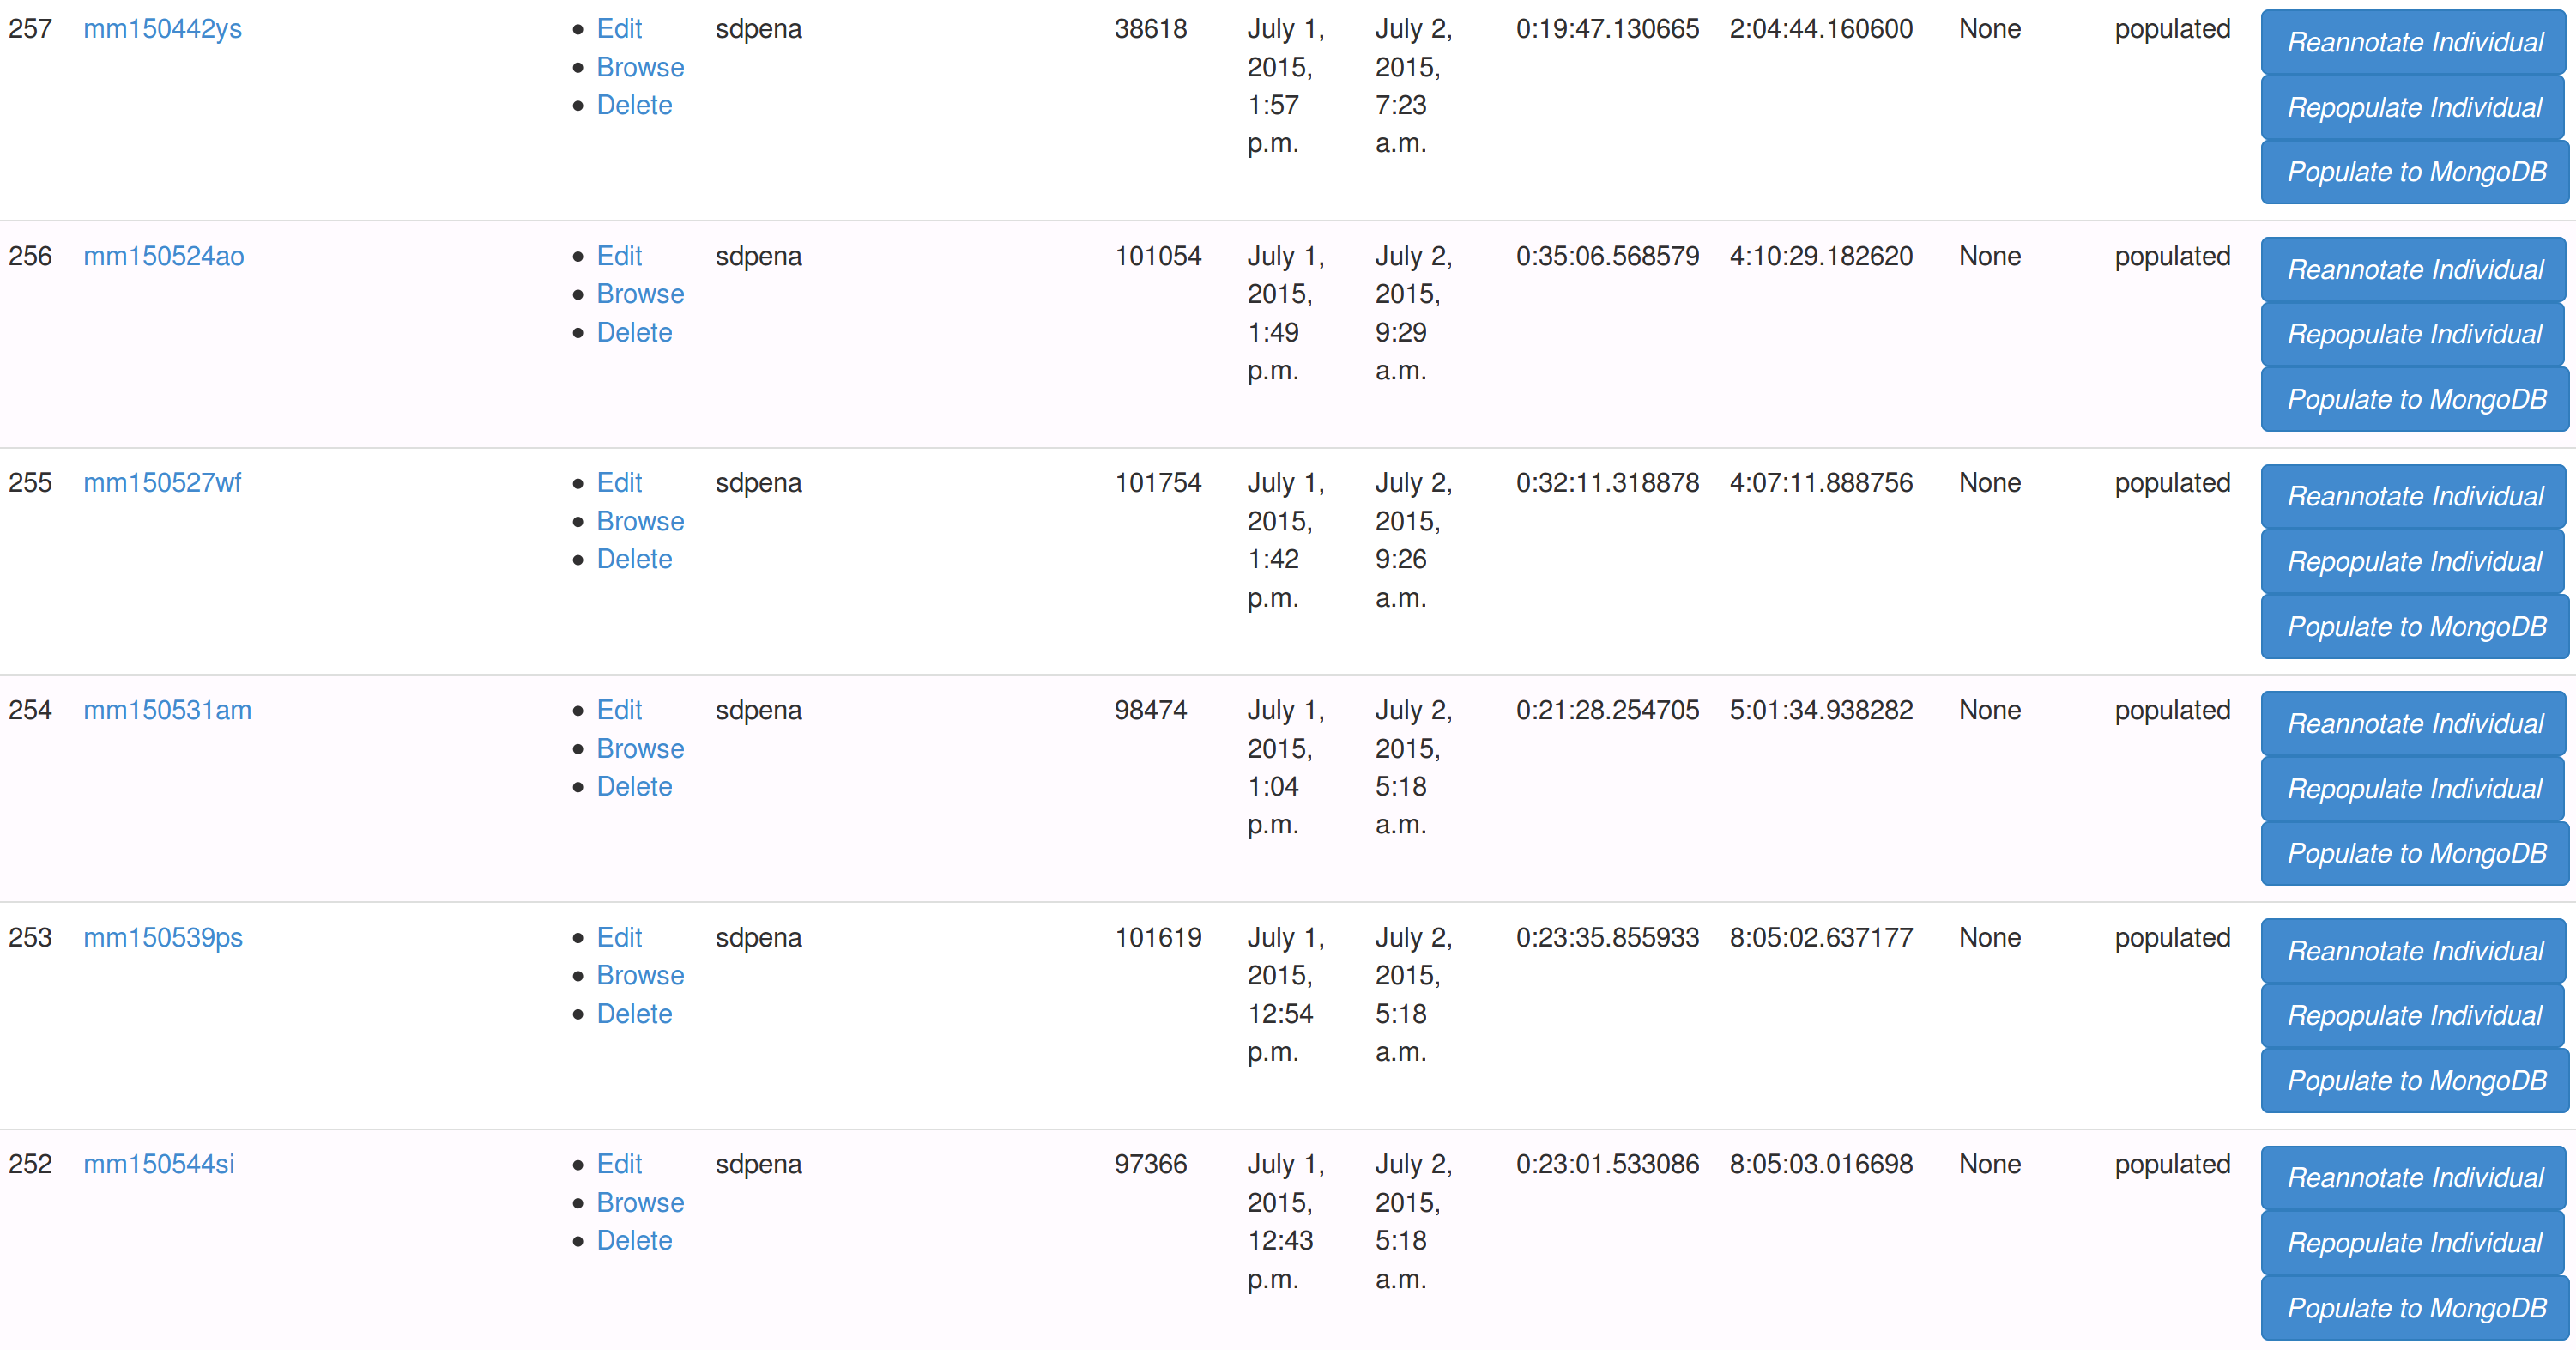
\includegraphics[width=1.3\textwidth]{./Figures/mendelmd/Dashboard.png}}
  \caption[Dashboard - Interface para visualização dos indivíduos no sistema]{A partir desta interface é possível visualizar as variantes de cada indivíduo, reanotar os indivíduos e reinserí-los no banco de dados. Da esquerda para a direita temos as colunas: ID, nome da amostra, usuário, número de variantes, Data da criação, data da modificação, tempo de anotação, tempo de inserção no banco de dados e estado da amostra.}
  \label{fig:dashboard}
\end{figure}
\end{landscape}

\clearpage
}


\subsection{Upload de Genomas}

A figura~\ref{fig:upload} apresenta a interface de submissão de indivíduos para o sistema. Essa interface foi desenvolvida utilizando a biblioteca de javascript chamada Jquery FileUpload e facilita o envio de arquivos VCFs para o sistema permitindo o upload simultâneo de indivíduos para o servidor usando para isso qualquer dispositivo (computador, tablet ou celular) que tenha acesso a internet.

\afterpage{
  \begin{landscape}
\begin{figure}[p]
  \centering
  \Large\textbf{Interface para submissão dos indivíduos no sistema}\par\medskip
  \fbox{\includegraphics[width=1.5\textwidth]{./Figures/mendelmd/upload.png}}
  \caption[Interface para submissão dos indivíduos no sistema]{A interface de submissão dos indivíduos foi desenvolvida utilizando a biblioteca Jquery FileUpload para facilitar essa tarefa.}
  \label{fig:upload}
\end{figure}
\end{landscape}
\clearpage
}


\subsection{Agendador de Tarefas}

O Celery é um sistema agendador de tarefas assíncronas e distribuídas que permite a integração e execução de diferentes scripts e programas. Este programa foi utilizado para permitir a anotação automática dos dados de maneira totalmente assíncrona a partir do momento que o usuário realiza o upload dos dados no sistema. Nas figuras~\ref{fig:celery_shell} e~\ref{fig:celery_annotation} apresentamos a interface do celery, na figura ~\ref{fig:celery_annotation} é possível verificar diversos scripts sendo executados em paralelo para realizar a anotação de um exoma que foi inserido no sistema.

\afterpage{
  \begin{landscape}
\begin{figure}[p]
  \centering
  \Large\textbf{Interface do Celery}\par\medskip
    \fbox{\includegraphics[width=1.5\textwidth]{./Figures/Celery_Shell.png}}
  \caption[Interface do Celery]{Nesta figura podemos visualizar a interface de comando do Celery. Nesta interface podemos verificar o output de cada programa utilizado durante a anotação de variantes.}
  \label{fig:celery_shell}
  \end{figure}
\end{landscape}

\clearpage
}


\afterpage{
  \begin{landscape}
\begin{figure}[p]
  \centering
  \Large\textbf{Processo de anotação de variantes}\par\medskip
  \fbox{\includegraphics[width=1.5\textwidth]{./Figures/Celery_annotation.png}}
  \caption[Processo de anotação de variantes]{Nesta figura podemos observar diversos scripts sendo executados em paralelo utilizando o Celery para realizar a anotação de exomas através do uso de diferentes programas como SnpEff e VEP.}
  \label{fig:celery_annotation}
  \end{figure}
\end{landscape}

  
  \clearpage
}

\subsection{Conversão dos dados para CSV}

Apesar do Mendel,MD ter sido criado para facilitar o processo de filtragem dos dados utilizando para isso uma interface web, nós também desenvolvemos um script em python para realizar a conversão dos dados de VCF para CSV após o término do processo de anotação. Além disso foi desenvolvido uma programa usando wxPython que permite a conversão entre arquivos do tipo VCF para CSV de maneira local utilizando para isso uma interface gráfica com janelas e botões. Isso permite que o usuário converta os dados de VCF para CSV para que eles possam ser filtrados manualmente pelo Médico ou Pesquisador usando um programa de planilhas, como por exemplo o Excel ou o Libre Office Calc.

A figura~\ref{fig:vcf2csv} apresenta a interface gráfica desenvolvida para realizar essa conversão entre os formatos VCF e CSV. Essa transformação entre os formatos também realiza a de-normalização dos dados presentes nas colunas INFO do VCF de maneira que todos os dados dessa coluna fiquem separados em colunas diferentes no arquivo CSV final.

Além disso, também foi adicionada uma opção para que o usuário pudesse alterar a ordem das colunas no arquivo de saída.

\afterpage{
\begin{landscape}

\begin{figure}[p]
  \centering
  \Large\textbf{Programa desenvolvido para conversão entre arquivos VCF e CSV}\par\medskip
  \fbox{\includegraphics[width=1.5\textwidth]{./Figures/vcf2csv.png}}
  \caption[Programa desenvolvido para conversão entre arquivos VCF e CSV]{Interface do programa desenvolvido para conversão entre os formatos VCF e CSV.}
  \label{fig:vcf2csv}
\end{figure}
\end{landscape}
\clearpage
}

\subsection{Anotação de Variantes}

Para realizar a integração de diferentes ferramentas e fontes de informação, foi desenvolvido um \textit{framework} que realiza toda a anotação das variantes e que integra a maior parte dos dados e ferramentas existentes relacionados a este tipo de análise. A figura \ref{fig:framework_anotacao} é a principal figura deste trabalho, onde é apresentado o \textit{framework} que foi desenvolvido durante este trabalho. Pode-se observar nesta figura todos os processos que ocorrem dentro do pipeline de anotação desenvolvido para o Mendel,MD.

Após a inserção dos indivíduos no sistema, nós primeiramente realizamos uma validação dos arquivos VCFs através de um método chamado ``\textit{vcf-validator}'' que faz parte do programa \textit{VCFTools}. Este método realiza diversos testes no arquivo VCF de entrada e ao final gera um arquivo com todos os problemas que foram encontrados. Após essa validação inicial o arquivo passa então por um método que desenvolvemos chamado de ``\textit{sanity-check}'' que prepara o arquivo VCF para ser anotado por diferentes ferramentas.

Uma das primeiras ferramentas integradas para a anotação dos dados foi o SNPEFF que entre outras coisas fornece informações importantes sobre cada mutação como por exemplo a classificação do seu impacto de acordo com as seguintes classes: MODIFIER, LOW, MODERATE e HIGH. Essas classes são extremamente úteis na hora de realizarmos a filtragem de variantes, o mais recomendado aqui seria primeiro fazer a busca em variantes que são MODERATE e HIGH pois aí estarão presentes as mutações que são mais graves e possivelmente podem causar uma alteração da estrutura de uma proteína.

Outro programa integrado pela nossa anotação foi o Variant Effect Predictor (VEP). Este programa realiza a anotação das variantes em relação aos tipos de mutações encontradas, aos aminoácidos que estão alterados, e caso ela seja uma mutação não-sinônima, anota a posição em relação ao cDNA. Além disso, o VEP também fornece escores de patogenicidade como por exemplo o SIFT e o Polyphen2 que são os escores mais utilizados atualmente quando buscamos por variantes patogênicas.

O banco de dados dbNFSP trouxe a capacidade de agregar centenas de informações diferentes para nossa análise como por exemplo anotação em relação a diferentes bancos de dados, escores de patogenicidade e de conservação de mutações. Para integrar essa ferramenta nós desenvolvemos um script em python chamado de ``\textit{pynnotator}'' que por sua vez utiliza bibliotecas como \textit{pysam} e \textit{parallel python} para realizar a anotação dos dados de uma maneira rápida eficiente, inclusive fazendo o uso de  múltiplos cores do processador ao mesmo tempo. Esse tipo de implementação não foi trivial mas ajudou bastante a diminuir o tempo necessário para se realizar a anotação de cada VCF contra uma grande quantidade de dados. O tempo médio de anotação para cada exoma enviado para o sistema é de apenas dez minutos.

\afterpage{
\begin{landscape}

\begin{figure}[p]
  \centering
  \Large\textbf{Framework de anotação de variantes}\par\medskip
 \fbox{\includegraphics[width=1.2\textwidth]{./Figures/mendelmd/annotation_pipeline.png}}
 \caption[Framework de anotação de variantes]{Este foi o framework de anotação de variantes desenvolvido durante este trabalho, ele realiza a integração de diversas ferramentas e bancos de dados diferentes através de scripts desenvolvidos em python para automatizar todo o processo.}
 \label{fig:framework_anotacao}
\end{figure}
\end{landscape}

\clearpage
}

\subsection{Controle de Qualidade sobre os dados}

Para se realizar o controle de qualidade sobre os dados foi desenvolvida uma interface para calcular e mostrar métricas de qualidade calculadas a partir dos VCFs de cada indivíduo. Na figura \ref{fig:individuals_view} podemos observar algumas o número de variantes homozigotas e heterozigotas (0/1 e 1/1). Além disso nesta seção é possivel verificar outras métricas como o número de variantes para cada indivíduo, a cobertura média de cada exoma, a qualidade média de suas variantes, o número de variantes por cromossomo, o número de variantes por classe funcional entre outras opções que são apresentadas.

\afterpage{
    \begin{landscape}
\begin{figure}[p]
  \centering
    \Large\textbf{Interface para visualizar métricas sobre os dados inseridos}\par\medskip
   \fbox{\includegraphics[width=1.5\textwidth]{./Figures/mendelmd/individuals_view.png}}
  \caption[Interface para visualizar métricas sobre os dados inseridos]{Nesta interface podes visualizar o número total de variantes, os tipos de variante encontradas no indivíduo e diversas outras métricas que são importantes para auxiliarem na filtragem de variantes como o número médio de qualidade e de cobertura para cada indivíduo.}
  \label{fig:individuals_view}
    \end{figure}
\end{landscape}


\clearpage
}

\subsection{Genes}

Na figura \ref{fig:genes_search} apresentamos a interface desenvolvida para realizar a busca de genes no sistema. Com essa interface é possível buscar genes por ``gene symbol'', por exemplo ``\textit{SUCLA2}'' ou então por uma parte do nome do gene ``succinate'' e então selecionar os genes obtidos nos resultados para serem utilizados no método de filtragem de variantes.

\afterpage{
  \begin{landscape}
\begin{figure}[p]
  \centering
  \Large\textbf{Interface para Busca de Genes}\par\medskip
  \fbox{\includegraphics[width=1.5\textwidth]{./Figures/mendelmd/genes.png}}
  \caption[Interface para Busca de Genes]{Essa interface foi desenvolvida para permitir a busca de genes específicos, após a obtenção do resultado é possível investigar variantes apenas na lista de genes desejada.}
  \label{fig:genes_search}
  \end{figure}
\end{landscape}


  \clearpage
}

Também foi desenvolvida um opção para armazenar listas de genes personalizadas como por exemplo, com genes que já estivessem associados com doenças Mendelianas dominantes e recessivas. A figura \ref{fig:gene_lists} apresenta as listas de genes que foram inseridas no Mendel,MD.

\afterpage{
  \begin{landscape}
\begin{figure}[p]
  \centering
  \Large\textbf{Interface com grupos de genes adicionados}\par\medskip
  \fbox{\includegraphics[width=1.5\textwidth]{./Figures/mendelmd/gene_lists.png}}
  \caption[Interface com grupos de genes adicionados]{Nesta interface podemos verificar os grupos de genes que foram criados pelos usuários de acordo com alguns critérios desejados.}
  \label{fig:gene_lists}
  \end{figure}
\end{landscape}

\clearpage
}

\subsection{Doenças}

Para obter dados sobre doenças Mendelianas nós utilizamos o site OMIM que possui atualmente 6845 doenças e 4715 genes. Esses dados foram inseridos no Mendel,MD para que fosse possível buscar por genes associados a doenças Mendelianas e para que eles pudessem ser inseridos no processo de filtragem de variantes.

Na figura \ref{fig:diseases} apresentamos a interface que permite a busca por doenças Mendelianas. Aqui é possível buscar por doenças e também selecionar os resultados para serem visualizados no método de filtragem de variantes na busca por variantes candidatas que estejam presentes nos indivíduos afetados pela doença. Nesta página o usuário pode digitar uma doença e selecionar todos os genes associados com ela para buscar variantes em seus indivíduos.

\afterpage{
  \begin{landscape}
\begin{figure}[p]
  \centering
  \Large\textbf{Interface para Busca de Doenças}\par\medskip
  \fbox{\includegraphics[width=1.5\textwidth]{./Figures/mendelmd/diseases.png}}
  \caption[Interface para Busca de Doenças]{Nesta interface podemos visualizar o resultado da busca por doenças com a palavra situs. A partir desta interface é possível visualizar variantes apenas em genes associados a um ou mais tipos específicos de uam determinada doença escolhida pelo usuário.}
  \label{fig:diseases}
  \end{figure}
\end{landscape}

\clearpage
}

\subsection{Filtragem de Variantes}

Após a anotação dos dados pelo sistema, o usuário pode filtrar as variantes dos indivíduos utilizando para essa tarefa um formulário web que permite a eliminação de variantes utilizando diferentes critérios de filtragem para tentar identificar a variante que possa ser responsável por causar a doença do paciente.

Este método foi implementado para permitir que essa tarefa pudesse ser repetida muitas vezes, facilitando a compreensão do que acontece durante cada etapa do processo e permitindo a combinação de diferentes opções de filtragem para chegar a uma lista pequena de candidatos.

As figuras a seguir ilustram o processo de filtragem implementado no Mendel,MD e que foram divididos em 3 etapas.
% 
% Step1Individuals.png
% Step2Variants.png
% Step3Databases.png
\afterpage{
  \begin{landscape}
\begin{figure}[p]
  \centering
    \Large\textbf{Filtragem de Variantes - 1ª Etapa}\par\medskip
    \fbox{\includegraphics[width=1.3\textwidth]{./Figures/Filtragem/Step1Individuals.png}}
  \caption[Filtragem de Variantes - 1ª Etapa]{Essa é a primeira tela da filtragem de variantes onde o usuário precisa selecionar as opções referentes aos indivíduos, genes e snps que deseja analisar.}
  \label{fig:filtering_step1}
  \end{figure}
\end{landscape}

\clearpage
}

A figura \ref{fig:filtering_step1} mostra a primeira etapa onde o usuário pode selecionar os indivíduos em que gostaria de visualizar as variantes existentes e também os indivíduos que gostaria que fossem utilizados como controles no processo de exclusão de variantes. Além disso o usuário pode utilizar uma lista de genes e SNPs que gostaria de incluir ou excluir nos indivíduos selecionados.

\afterpage{
  \begin{landscape}
\begin{figure}[p]
  \centering
    \Large\textbf{Filtragem de Variantes - 2ª Etapa}\par\medskip
    \fbox{\includegraphics[width=1.5\textwidth]{./Figures/Filtragem/Step2Variants.png}}
  \caption[Filtragem de Variantes - 2ª Etapa]{Nesta interface é possível selecionar algumas opções das variantes presentes nos arquivos VCF.}
  \label{fig:filtering_step2}
  \end{figure}
\end{landscape}

\clearpage
}


Na figura \ref{fig:filtering_step2} apresentamos a segunda etapa onde o usuário possui diversas opções para definir sobre o tipo de variante que gostaria de visualizar nos resultados. A primeira opção seria em relação ao tipo de variante homozigótica (Ex. 1/1, 2/2 e 3/3) ou heterozigótica (Ex. 0/1, 0/2 e 0/3), esses números correspondem ao genótipos que foram codificados no arquivo VCF para cada indivíduo. Existe uma opção que foi desenvolvida para selecionar apenas variantes em um único cromossomo ou então em uma região específica de um cromossomo como por exemplo: chr:17, pos:80789468-80789469. Isso pode ajudar na investigação de regiões homozigóticas onde possam existir variantes candidatas.

Nesta aba o usuário também pode selecionar o tipo da mutação, o cromossomo, a posição, a coluna de filtro do VCF (Ex. PASS, LowQual), o efeito da variante, a classe funcional, o impacto, o dbSNP Build de quando a variante foi inserida no dbSNP, a cobertura, a qualidade, o número de variantes por gene, exibir apenas variantes presentes em genes comuns entre os indivíduos selecionados, mostrar apenas variantes que não estejam presentes no dbSNP, mostrar apenas variantes anotadas como \textit{``clinically associated''} pelo clinvar e também excluir variantes presentes em regiões com segmento de duplicação


\afterpage{
  \begin{landscape}
\begin{figure}[p]
  \centering
    \Large\textbf{Filtragem de Variantes - 3ª Etapa}\par\medskip
    \fbox{\includegraphics[width=1.5\textwidth]{./Figures/Filtragem/Step3Databases.png}}
  \caption[Filtragem de Variantes - 3ª Etapa]{Nesta interface é possível selecionar valores em relação aos Bancos de Dados e Escores de Priorização que foram anotados para cada variante.}
  \label{fig:filtering_step3}
  \end{figure}
\end{landscape}

\clearpage
}

Conforme apresentado na figura \ref{fig:filtering_step3}, a terceira etapa permite a filtragem utilizando valores de máximo e mínimo da frequência possível das variantes em bancos de dados como 1000Genomes, dbSNP e ESP6500. Por último foram incluídos filtros para se eliminar variantes utilizando os escores de SIFT e Polyphen-2.

Além disso, também é possível utilizar outras opções como por exemplo, apenas genes relacionados a doenças específicas do OMIM. Ao começar a digitar, usamos uma função \textit{autocomplete} que foi desenvolvida usando uma biblioteca de Javascript chamada de Select2 que retorna uma lista de doenças para que o usuário possa adicionar em suas pesquisa. Isso facilita muito a investigação de doenças que possuam um fenótipo parecido mas que sejam causadas por genes diferentes. Rapidamente podemos adicionar diversos nomes de doenças na pesquisa que o sistema irá encontrar apenas os genes relacionados a estas doenças. 

\subsubsection{1-Click}

Nesta interface foi desenvolvida uma configuração padrão de filtros que são recomendados para o início do processo de filtragem de variantes. Esta interface foi desenvolvida para facilitar e automatizar a identificação de variantes causadoras de doenças Mendelianas.

O método 1-Click foi inspirado em uma opção da ferramenta de análise filogenética Phylogeny.fr e permite que o usuário selecione apenas os indivíduos da análise e o tipo de herança genética mais provável o que reduz drasticamente o número de variantes candidatas para tentar encontrar a real causadora da doença do indivíduo. Este método faz com que os filtros sejam configurados automaticamente para o usuário. Esses valores foram definidos de maneira empírica e são apenas uma sugestão sobre como realizar a configuração dos filtros.

As configurações pré-definidas estão listadas a seguir:

\begin{itemize}
  \item SnpEff Impact: HIGH ou MODERATE
  \item Profundidade de Leitura maior ou igual a 10
  \item Mostrar apenas variantes em genes comuns aos indivíduos selecionados
  \item Excluir Variantes presentes no banco VariSNP
  \item Frequência da variante no 1000Genomes menor que 0.005
  \item Frequência da variante no dbSNP137 menor que 0.005
  \item Frequência da variante no Exome Variant Server menor que 0.005
\end{itemize}

\subsubsection{Análise de Filtros para Famílias}

Este método permite a análise de famílias (Ex. Trios, Quartetos e etc) que podem ser utilizadas no processo de filtragem para encontrar variantes que sejam heterozigóticas nos pais dos indivíduos e que sejam homozigóticas nos filhos afetados. Isso também permite a identificação de variantes candidatas que tenham um padrão de herança chamado de heterozigoto composto, ou seja, quando o filho recebe um alelo do gene com defeito de cada um dos pais. Além disso esta opção também permite a visualização de variantes chamadas \textit{de novo}, ou seja, aquelas que estão presentes nos filhos mas que obrigatoriamente não estejam presentes em nenhum dos pais selecionados.

Para isso nós desenvolvemos uma interface onde é possível definir quem são os pais dos pacientes durante a análise. Então este método usa essa informação obtida para eliminar as variantes que estejam presentes nos pais e que não obedeçam aos critérios de herança estabelecidos. Na figura \ref{fig:family_analysis} podemos observar o formulário para este tipo de análise, e na figura \ref{fig:family_analysis_results} podemos verificar que nos resultados para cada genótipo encontrado nos filhos existe o genótipo de cada um dos pais. Quando selecionamos por exemplo a opção 'heterozigoto composto' o que acontece por trás é que o sistema mostra nos resultados apenas genes candidatos que possuem pelo menos uma variante de cada um dos pais. Esse tipo de análise ajuda muito a reduzir o número de genes candidatos.


\afterpage{
\begin{landscape}
\begin{figure}[p]
  \centering
    \Large\textbf{Interface do Family Analysis}\par\medskip
  \fbox{\includegraphics[width=1.5\textwidth]{./Figures/mendelmd/family_analysis.png}}
  \caption[Family Analysis]{Family Analysis - Neste formulário é possível selecionar quem são os pais dos indivíduos que estão sendo analisados para usar essa informação na hora da filtragem de dados}
  \label{fig:family_analysis}
\end{figure}
\clearpage
\end{landscape}
}




\afterpage{
\begin{landscape}
\begin{figure}[p]
  \centering
    \Large\textbf{Resultado do Family Analysis}\par\medskip
    \fbox{\includegraphics[width=1.5\textwidth]{./Figures/mendelmd/family_analysis_results.png}}
  \caption[Resultado do Family Analysis]{Nos resultados do Family Analysis é possível visualizar o genótipo de cada um dos pais para cada indivíduo nos resultados da análise}
  \label{fig:family_analysis_results}
\end{figure}
\end{landscape}

\clearpage
}
% 
% \subsubsection{Filter Pathway Analysis}
% 
% Este método mostra as variantes do resultado agrupadas por vias metabólicas do Kegg.  Isso permite a busca por variantes que estejam possivelmente associadas com uma única via metabólica. Para validar esta técnica utilizamos duas doenças chamadas Síndrome de \textit{Hurler} e de \textit{Hunter} que são causadas por mutações em genes diferentes (IDUA e IDS) mas que ambos os genes pertencem a via metabólica de glicosaminoglicanos. Na figura \ref{fig:pathway_analysis} podemos verificar que os resultados da análise estão agrupados por vias metabólicas. 
% 
% \afterpage{
% \begin{figure}[p]
%   \centering
%   \caption[Pathway Analysis]{Pathway Analysis - O resultado da filtragem aparece agrupado por vias metabólicas do KEGG}
%     \includegraphics[width=1.0\textwidth]{./Figures/mendelmd/pathway_analysis.png}
%   \label{fig:pathway_analysis}
% \end{figure}
% \clearpage
% }

\subsubsection{Visualização de variantes}

Ao encontrar uma variante de interesse é possível verificar todas as informações disponíveis sobre aquela variante no sistema clicando no botão ''View``. Para isso nós desenvolvemos uma interface que mostra todos os campos do banco de dados para aquela variante específica. Esta interface possui centenas de anotações para cada variante.

\subsubsection{Exportação de resultados}

Após o usuário realizar a filtragem dos dados do paciente é possível exportar as variantes restantes em formato csv clicando sobre o botão ''\textit{export to csv}`` para que elas possam ser investigadas manualmente por um clínico utilizando programas como por exemplo o Excel.

\subsection{Comparação de Exomas}

Para possibilitar a comparação de exomas de diferentes indivíduos e até mesmo de exomas do mesmo indivíduo gerados a partir de tecnologias diferentes foi desenvolvido um método de comparação de VCFs. O algoritmo implementado nesta comparação possui duas etapas: primeiro procura apenas por posições que sejam comuns aos dois indivíduos sendo comparados, depois verifica se o genótipo nessas posições é igual ou diferentes entre os dois arquivos.

Na figura \ref{fig:comparison} podemos observar a comparação do genótipo de dois irmãos (Exome\_2\_MB e Exome\_3\_EDS) através deste método. Nesta caso nós encontramos 48.110 variantes em posições em comum entre os dois irmãos sendo que 84.2\% dessas variantes tinham o mesmo genótipo nos dois indivíduos selecionados.

\afterpage{
\begin{landscape}
\begin{figure}[p]
  \centering
    \Large\textbf{Interface para comparação de indivíduos}\par\medskip
  \fbox{\includegraphics[width=1.3\textwidth]{./Figures/mendelmd/comparison.png}}
  \caption[Interface para comparação de indivíduos]{Essa interface foi desenvolvida para permitir a comparação de dois indivíduos ou VCFs.}
  \label{fig:comparison}
\end{figure}
\end{landscape}

\clearpage
}